\chapter{Lexicalized domain representation}
\section{Motivation}
  We study here \emph{supervised multi-domain adaptation} setting \ref{sec:case1}, where the number of domains is potentially large and adapting separately to each domain would waste training resources. Our proposal transposes to neural machine translation the feature expansion technique of (Daum\'e III, 2007): it isolates domain-agnostic from domain-specific lexical representations, while sharing the most of the network across domains.
  
Our experiments use two architectures and two language pairs: they show that our approach, while simple and computationally inexpensive, outperforms several strong baselines and delivers a multi-domain system that successfully translates texts from diverse sources.

We adapt here ideas of \cite{Daume07frustratingly} to neural MT. Our main hypothesis is that domains mostly differ at the lexical level, due to cross-domain polysemy, which motivates domain specific embeddings. By contrast, the deeper layers, which arguably model more abstract linguistic phenomena, are made shareable across domains. To this end, we design word embeddings containing a generic and several domain-specific regions. We experiment with four domains, two neural architectures and two language pairs and find that our technique yields effective multi-domain NMTs, outperforming several baselines. Our contributions are thus as follows: we adapt and implement the ideas of \cite{Daume07frustratingly} for two NMT architectures; we provide experimental evidence that show the effectiveness of this technique; we evaluate the ability of our networks to dynamically accommodate new domains; and we introduce a new technique to analyze word polysemy using embeddings, which comforts the assumption that their variation across domains actually reflects a variation of senses.

\section{Lexicalized domain representations\label{sec:lexicalized_embeddings}}
\subsection{Multi-domain machine translation \label{ssec:statement}}

Multi-domain machine translation is formalized as follows: we assume observations taking the form of  domain-tagged sentence pairs $[(x,y),i]$, with $x$ in the source language, $y$ in the target language and $i$ a domain tag in $[1\dots d]$. We further assume a two-stage sampling process: first select a domain $i$ according to $p(i)$, then select a sentence pair according to a domain specific distribution $D_i$. Our objective is to find a tuple of parameters $\{\theta_1 \dots \theta_d \} \in \mathbb{R}^D \times \dots \times \mathbb{R}^D$ minimizing:
\begin{equation} \label{eq:loss}
\begin{split}
\sum_{i \in [1..d]} p(i) E_{(x,y) \sim D_{i}} [-log(p_{\theta_i}(y|x,i))] \text{.}
\end{split}
\end{equation}
The training data for domain $i$ is denoted $C_i$.

A straightforward solution is to process each domain separately, computing the value $\theta_i^*$ that minimizes the empirical loss on $C_i$. This strategy is only effective if we have sufficient training data for each domain; when this is not the case, some estimates $\theta_i^*$ may be far from their optimal value. \fyDone{Risk}
The alternative we consider here constraints each parameter $\theta_i$ to be made of two parts: $\theta_i = [\theta_s; \theta'_i]$. $\theta_s \in R^{D_g}$ is shared across all domains, while the second part $\theta'_i \in \mathbb{R}^{D_i}$ is only used in domain $i$.
The parameter set is now much more constrained, yet we expect that tying parameters across domains will yield better estimates for $\theta_s$ due to a larger training corpus. In this setting, the optimization program defined by equation~\eqref{eq:loss} can no longer be performed separately for each training corpus.

\subsection{Lexicalized domain embeddings \label{ssec:lde}}

To actually implement this idea for NMT, we need to define the subset of parameters that will be shared across domains. 
Our hypothesis is that domain specificities can be confined to the lexical level and we define $\theta_s$ to contain all the network parameters except for a subpart of the word embeddings. 
For each word $v$, the embedding vector $e(v)$ is thus decomposed as $e(v) = [e_g(v); e_1(v); \dots; e_d(v)]$, where $e_g(v)$ stores the generic lexical embedding, while $e_i(v)$ stores the subpart that is specific to domain $i$.
In our NMT architectures, the actual embedding layer composes these vectors linearly to generate the word embedding for domain $k$ according to:

\begin{align}
  \tilde{e}_k(v) =& M_g e_g(v) + \sum_{i \in [1,..,d]} M_i \times e_i(v) \times \delta(i=k) \nonumber \\
   & = M [e_g(v); e_1'(v,k) \dots; e_d'(v,k)], \label{eq:embedding}
\end{align}
where $\delta()$ is the indicator function, $M$ is the matrix made of blocks $M_g, M_1 \dots, M_d$, and $e_i'(v,k)$ is the masked embedding: $e_i'(v,k)= e_i(v) * \delta(i=k)$.  

\begin{figure}[h]
  \center
  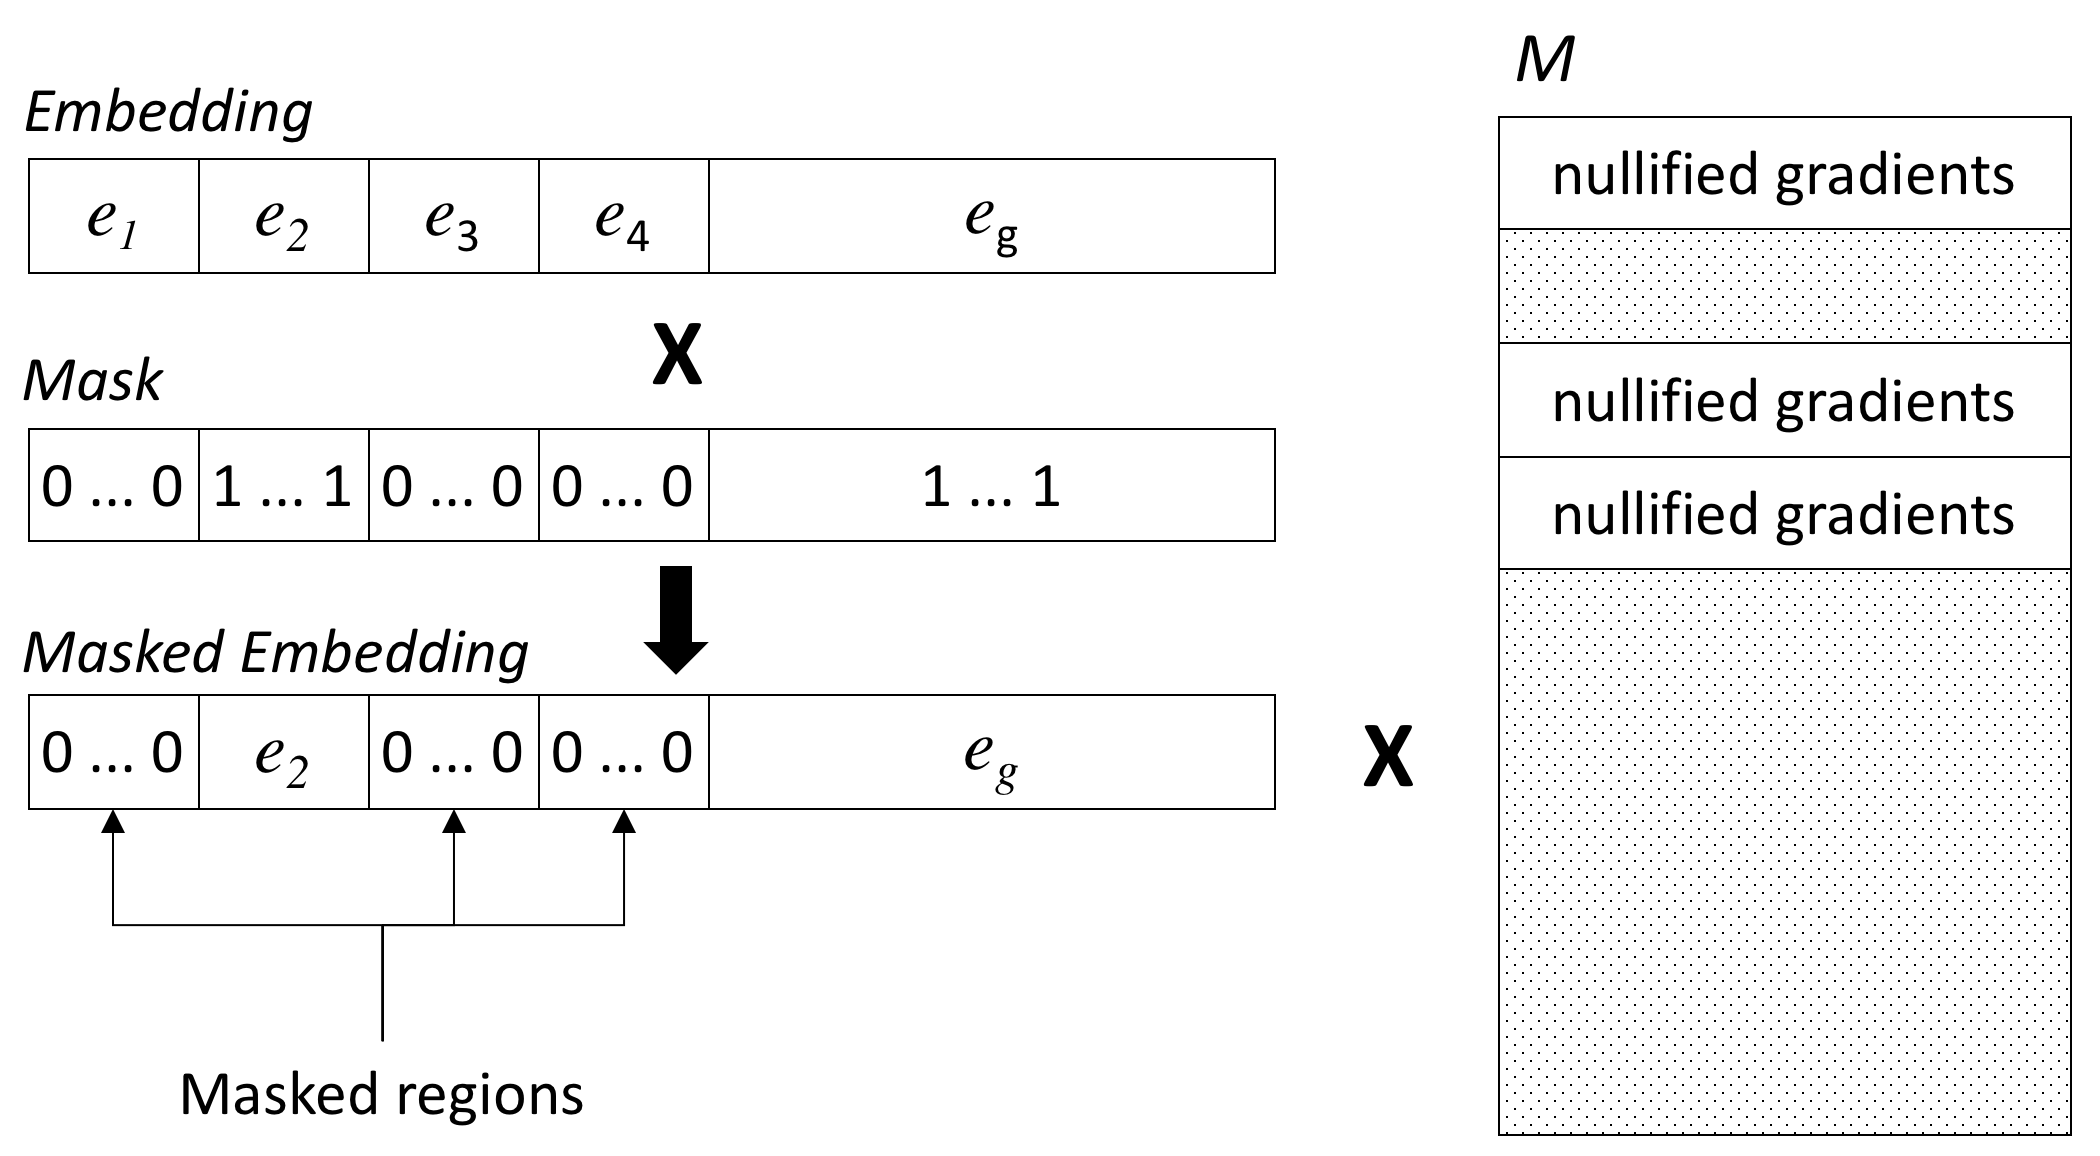
\includegraphics[width=0.48\textwidth]{graphics/embeddings}
  \caption{Lexicalized domain embeddings. When processing a sample from domain $2$, we only activate the corresponding parameter region ($\theta_2$) in the input embeddings; the remaining domain-specific parts are zeroed out and do not receive any update. The generic part is always active and is updated irrespective of the input domain.} 
  \label{fig:network}
\end{figure}

Making sure that the actual embedding do not contain any zero is important for the Transformer model, since the lexical representations are then added to the positional encoding, which would undo the effect of domain masking, and propagate a gradient even to regions that should not be modified. 
With our design, we make sure that during backprogation, the matrix $M$ receives gradient $0$ at regions corresponding to deactivated regions in the word embedding. 
Those regions are also masked in forward step, thus do not interfere the training on the domains to which they are not assigned (see Figure~\ref{fig:network}).
%
Our architecture is thus readily compatible with any NMT architecture, where we simply replace standard embedding layers 
by the embeddings defined
in equation~\eqref{eq:embedding}. In our experiments, we consider both the attentional RNN architecture of \cite{Bahdanau15learning} and the Transformer architecture of \cite{Vaswani17attention}.

\section{Experiments \label{sec:experiments}}

\subsection{Domains and data \label{ssec:data}}

We experiment with two language pairs (English-French, English-German) and data originating from three domains, corresponding to texts from three European institutions: 
the European Parlement (EPPS) \cite{Koehn05europarl}, 
the European Medicines Agency (EMEA), 
the European Central Bank (ECB) \cite{Tiedemann09news},
In addition, for English-French we also use IT-domain corpora obtained from the OPUS web site\footnote{\url{http://opus.nlpl.eu}} corresponding to KDE, Ubuntu, GNOME and PHP datasets (IT).
%
We randomly split those corpora into training, validation and test sets (see statistics in Table~\ref{tab:Corpora}).
Validation sets are used to chose the best model according to the average BLEU score \cite{Papineni02bleu}.
%Using internal test sets corresponds to somewhat ideal conditions.

%for contrast experiments, we also use supplementary test sets from three other domains: the official Khresmoi testset \cite{Khresmoi17test}, which is close to EMEA, News test 2014 \cite{Bojar14findings}, and IWSLT 2010 (Talk track) \cite{Paul10overview}. This enables us to evaluate the loss in performance when the test set is from a domain not seen in training.
% The model is also required to achieve comparable performance to generic model. To do so, we use newstest 2009 and IWSLT 2010 whose contain does not particularly belong to any domain.

\fyDone{Check which corpus are useful}
\begin{table}[h]
  \centering
  \begin{tabular}{ |llll|} %*{4}{|r|}}
    \hline
    Corpus & Train & Valid & Test \\ 
    \hline
    \multicolumn{4}{l}{English $\rightarrow$ French }\\
    %\multicolumn{4}{|l|}{Vocab size - En: 30,165, Fr: 30,398}\\
    \hline
    EMEA  & 1.09M & 1,000 & 1,000$_{(300)}$\\
    ECB    & 0.19M & 1,000 & 1,000     \\
    EPPS   & 2.01M  & 1,000 & 1,000  \\
    IT         & 0.54M  & 1,000 & 1,000 \\  
    \hline
    \multicolumn{4}{l}{English $\rightarrow$ German}\\
    %\multicolumn{4}{|l|}{Vocab size -  En:30,159, De: 30,698}\\ 
    \hline
    EMEA  & 1.11M & 1,000 & 1,000$_{(300)}$ \\
    ECB     &  0.11M & 1,000 & 1,000  \\
    EPPS   & 1.92M & 1,000 & 1,000 \\ 
    \hline
\end{tabular}
\caption{Corpora statistics.}
\label{tab:Corpora}
\end{table}

Note that the EMEA dataset distributed on the OPUS site contains multiple sentence duplicates. 
We therefore report below two numbers as $S_{(T)}$: the first ($S$) is comparable to what has been published on earlier studies (eg.\ \cite{Zeng18multidomain}), the second one ($T$) is obtained by making the test entirely disjoint from the training (700~duplicated sentences are discarded).

To reduce the number of lexical units and make our systems open-vocabulary, we apply Byte-Pair Encoding \cite{Sennrich16neural} separately for each language with 30,000 merge operations. \fyDone{I need explanations here}

\subsection{Baselines \label{ssec:baselines}}
To validate our findings, we compared lexicalized domain embedding models with standard models using both attentional Recurrent Neural Networks (RNNs) \cite{Bahdanau15learning} and the Transformer architecture of \cite{Vaswani17attention}. Our baselines consist of:
\begin{itemize}
\item generic models trained with a simple concatenation of all corpora (\texttt{Mixed});
\item models tuned separately on each domain for respectively (10000, 15000, 5000) iterations using in-domain data (\texttt{ft$_{EMEA}$}, \texttt{ft$_{EPPS}$}, \texttt{ft$_{ECB}$}); 
\item models using domain tags as in \cite{Kobus17domain} (\texttt{DC}); 
\end{itemize}

For all models, we set the embeddings size equal to 512; the size of hidden layers is equal to 1024 for RNNs and 512 for Transformer. 
Other important configuration details are as follows:
Transformer models use multi-head attention with 8 heads in each of the 6 layers; 
the inner feedforward layer contains 2048 cells;  
RNN models use 1 layer on both sides: 
a bidirectional LSTM encoder and a unidirectional LSTM decoder with attention.
The domain control systems are exactly as their baseline counterparts (RNN and Transformer), with an additional 2 cells encoding the domain on the input layer.
 %
To train NMT systems, we use Adam, with parameters $\beta_1=0.9$, $\beta_2 = 0.999$, $\alpha=0.0005$ for RNNs; with parameters $\beta_1=0.9$, $\beta_2= 0.98$, with Noam decay \cite{Vaswani17attention} for Transformer ($warmup\_steps=4000$). In all cases, we use a batch size of~128 and a dropout rate of 0.1 for all layers. 
All our systems are implemented in OpenNMT-tf\footnote{\url{https://github.com/OpenNMT/OpenNMT-tf}} \cite{Klein17opennmt}.

\subsection{Implementing Lexicalized Domain Representations}\fyDone{Check acronym.}

\fyDone{Motivate the split - discuss experimentally embedding size}
In order to implement lexicalised domain representations (henceforth \texttt{LDR}), we split the embedding vector into four regions: 
3 are domain specific and 1 is generic, with sizes $[8,8,8,488]$ respectively. %, a choice that will be discussed in Section~\ref{secc:region_size}. 
If a sentence originates from domain $i$, the domain specific regions for all domains $j \neq i$ will be zeroed out while the other regions are activated (cf. Figure~\ref{fig:network}). 
We then use a dense layer of size~512 to fuse the region for the active domain and the ``generic'' region. Training is formalised in algorithm~\ref{alg:multidomain}.
%
Note that each iteration of algorithm \ref{alg:multidomain} uses 2~batches: a ``generic'' batch updating only the generic region; and a ``domain-specific'' batch updating just the domain-specific parameters. 

\begin{algorithm}[h]
\caption{Multi-domain Training}
\label{alg:multidomain}
\begin{algorithmic}[1]
\REQUIRE {Corpora $C_i, i\in [1,..,d]$ for $d$ domains, Batch size $B$}%, Optimization algorithm $\operatorname{Opt}$}
\REPEAT 
\STATE{Randomly pick $i \in [1,..,d]$ w.r.t the multinomial distribution $[\frac{|C_i|}{\sum_{i\in [1,..,d]}|C_i|}]$.}
\STATE{Randomly pick $B$ sentences from $C_i$.}
\STATE{Activate only generic region to create generic batch, denoted $W_g$.}
% \STATE{Pass the generic embedding batch to a dense layer.}
\STATE{Compute gradient of $\theta_s$, $\frac{\partial L}{\partial \theta_s}$ using $W_g$.}
\STATE{Activate domain-specific and generic regions to create domain-specific batch $W_i$}
% \STATE{Pass $W_i$ to a dense layer}
\STATE{Compute gradient of domain-specific parameters $\theta_i$, $\frac{\partial L}{\partial \theta_i}$ using $W_d$.}
\STATE{Update parameters $\theta_s$ using $\frac{\partial L}{\partial \theta_s}(W_g)$ and $\theta_i$ using $\frac{\partial L}{\partial \theta_i}(W_i)$}
% $$ \theta_s = \theta_s - \operatorname{Opt}(\frac{\partial L}{\partial \theta_s}(W_g))$$ 
% $$ \theta_i = \theta_i - \operatorname{Opt} (\frac{\partial L}{\partial \theta_i}(W_i))$$}
\UNTIL{convergence}
\end{algorithmic}
\end{algorithm}


The batch selection procedure (step~2 of algorithm~\ref{alg:multidomain}) ensures that the number of examples of each domain used in training  follows the distribution of the training data.
%each domain is represented according to its frequency in the training data. 
In our experiments, this means that sentences from the Europarl domain will be selected more frequently that the two other domains. We also consider a more balanced sampling procedure, where $i$ is selected according to  distribution $[\frac{\sqrt{|C_i|}}{\sum_{i\in [1,..,d]}\sqrt{|C_i|}}]$.
The corresponding results are reported as \texttt{LDR}$^{0.5}$.
\subsection{Results \label{ssec:results}}

Results are summarized respectively in Table~\ref{tab:results-trsf} for the Transformer systems and Table~\ref{tab:results-rnn} for the RNN systems, where we report BLEU~\cite{Papineni02bleu} scores computed after detokenization.\footnote{As explained above, we  report two numbers when testing with EMEA, except for the fine-tuning scenarios when tuning on ECB and EPPS.} % \fyTodo{Footnote for missing numbers}.

%We first concentrate on the left part of these tables, where we analyze the performance for the three domains of interest. 
First, we observe that Transformer is consistently better than RNNs and that fine-tuning on a domain-specific corpus, when applicable, is almost the best way to optimize the performance on that domain.\footnote{This is not so clear for EPPS, where fine-tuning does not seem to help.}  
Note that fine-tuning however yields a marked (even sometimes catastrophic, eg.\ for the EMEA-tuned Transformer system) decrease in performance for the other domains. 

Our approach (\texttt{LDR}$_{oracle}$) is consistently better than the \texttt{Mixed} strategy, with gains that range from very large (for EMEA and ECB) to unsignificant (for EPPS in most conditions). 
This means that our architecture is somehow able to compensate for the data unbalance and to raise the performance of the multi-domain system close to the best (fine-tuned) system in each domain. 
We even observe rare cases where the \texttt{LDR}$_{oracle}$ system outperforms fine-tuning (eg.\ Transformer en:de in the EMEA domain). 
\texttt{LDR}$_{oracle}$ is also better than Domain Control in three conditions out of four, \texttt{DC} being seemingly a better choice for the RNN than for the Transformer architecture. 
As expected, ignoring the true domain label yields a light drop in performance: this is reflected in the results of %for the two fallback strategies considered in this study. 
%The first, \texttt{LDR}$_{generic}$, only uses the generic part of the embeddings. 
%The second, 
\texttt{LDR}$_{pred}$, which relies on automatically predicted domain labels.\footnote{Our domain classifier uses a bi-LSTM RNN encoder, followed by a simple softmax layer. 
Its precision on a development set exceeds 95\%.}
% \fyDone{Explain how}
Note that this decrease is however hardly significant, showing that our architecture is quite robust to noisy labels. 
Even in the worst case scenario where all domain tags are intentionally wrong (\texttt{LDR}$_{wrong}$), we see that the generic part still ensures a satisfying level of performance. 
A last contrast is with \texttt{LDR}$_{oracle}^{0.5}$ where we change the distribution of training sentences to decrease the weight of EPPS data and increase the number of ECB samples. 
As a result, we see a small decrease for EMEA and EPPS, and a large boost for ECB. 
This shows that our technique can be used in conjunction to other well known strategies for performing domain adaptation. 

\begin{table}[!h]
\begin{center}
\scalebox{1.0}{
\begin{tabular}{|l|lcc|c|}
\hline
Model & EMEA & EPPS & ECB & Avg. \\
\hline
%\multicolumn{8}{l}{} \\[-9pt]  
\multicolumn{5}{l}{English$\rightarrow$French} \\
\hline
$\mathtt{Mixed}$          & 67.69$_{47.60}$ & 37.50 & 53.49 & 52.89\\
\hline
$\mathtt{FT}_{EMEA}$ & 76.77$_{49.43}$ & 17.16 & 11.99 & 35.30\\
$\mathtt{FT}_{EPPS}$  & 20.86 & 37.04 & 24.53 & 27.47\\
$\mathtt{FT}_{ECB}$    & 26.93 & 27.09 & \bf 56.52 & 36.84\\
\hline
$\mathtt{DC}$              & 67.87$_{45.42}$ & 37.31 & 54.14 & 53.10\\
\hline
$\mathtt{LDR}_{oracle}$            & 74.26$_{\bf 49.90}$ & 37.67 & 54.07 & 55.33\\
$\mathtt{LDR}_{oracle}^{0.5}$   & \bf 74.95$_{49.38}$ & 37.35 & 55.91 & \bf 56.07\\
%$\mathtt{LDR}_{generic}$          & 73.97$_{49.54}$ & 37.81 & 53.67 & \\
$\mathtt{LDR}_{pred}$               & 74.29$_{49.84}$ & \bf 37.73 & 54.01 & 55.34\\
$\mathtt{LDR}_{wrong}$            & 72.95$_{49.78}$ & 37.62 & 53.35 & 54.64\\
  \hline
%\multicolumn{8}{l}{} \\[-9pt]
\multicolumn{5}{l}{English$\rightarrow$German} \\
\hline
$\mathtt{Mixed}$         & 64.57$_{42.99}$ & 26.47 & 68.67 & 53.23\\
\hline
$\mathtt{FT}_{EMEA}$ & 68.35$_{42.97}$ & 17.02 & 32.87 & 39.41\\
$\mathtt{FT}_{EPPS}$  & 36.19 & 26.29 & 40.71 & 34.39\\
$\mathtt{FT}_{ECB}$   & 24.72 & 18.36 & \bf 74.05 & 39.04\\
\hline
$\mathtt{DC}$ & 63.48$_{42.98}$ & 26.27 & 66.95 & 52.23\\
\hline
$\mathtt{LDR}_{oracle}$ & 70.90$_{\bf 46.12}$ & 26.30 & 68.90 & 55.36\\
$\mathtt{LDR}_{oracle}^{0.5}$ & \bf 71.31$_{45.23}$ & 25.98 & 73.74 & \bf 57.01\\
%$\mathtt{LDR}_{generic}$ & 70.86$_{45.60}$ & 26.14 & 68.59 & \\
$\mathtt{LDR}_{pred}$ & 70.89$_{\bf 46.12}$ & \bf 26.53 & 68.63 & 55.35\\
$\mathtt{LDR}_{wrong}$ & 69.51$_{43.50}$ & 26.31 & 66.86 & 54.22\\
\hline
\end{tabular}
} %scalebox
\end{center}
\caption{BLEU scores for  Transformer systems \label{tab:results-trsf}}
\end{table}

\begin{table}[!h]
\begin{center}
\scalebox{1.0}{
\begin{tabular}{|l|lcc|c|}
\hline
Model & EMEA & EPPS & ECB & Avg. \\
\hline
%\multicolumn{8}{l}{} \\[-9pt]
\multicolumn{5}{l}{English$\rightarrow$French} \\
\hline
$Mixed$                         & 65.42$_{45.11}$ & 34.70 & 51.38 & 50.50\\
\hline
$\mathtt{FT}_{EMEA}$   & 72.06$_{\bf 47.33}$ & 18.62 & 16.78 & 35.82\\
$\mathtt{FT}_{EPPS}$    & 35.47$ $ & 34.61 & 39.56 & 36.55\\
$\mathtt{FT}_{ECB}$      & 21.93$ $ & 22.60 & 51.53 & 32.02\\
\hline
$\mathtt{DC}$                            & 68.26$_{43.76}$ & 35.13 & 50.09 & 51.16\\
% \hline
%$\mathtt{WDCMT}$           & 68.76$_{45.29}$ & 35.71 & 52.75 & \\
\hline
$\mathtt{LDR}_{oracle}$            & 71.73$_{46.30}$ & \bf 35.21 & 50.91 & 52.62\\
%$\mathtt{LDR_{condgru}}_{pred}$   & 71.7$_{46.21}$ & 35.09 & 51.22 & \\
$\mathtt{LDR}_{oracle}^{0.5}$   & 71.70$_{46.41}$ & 34.24& \bf 52.37 & \bf 52.77\\
%$\mathtt{LDR}_{generic}$          & 70.59$_{46.37}$ & 35.22 & 49.68 & \\
$\mathtt{LDR}_{pred}$               &\bf 72.76$_{46.35}$ & 35.10 & 50.38 & 52.75\\
$\mathtt{LDR}_{wrong}$            & 62.10$_{43.29}$ & 34.17 & 48.79 & 48.35\\
\hline
%\multicolumn{8}{l}{} \\[-9pt]
\multicolumn{5}{l}{English$\rightarrow$German} \\
\hline
$Mixed$                        & 57.37$_{37.94}$ & 23.10 & 63.54 & 48.00\\
\hline
$\mathtt{FT}_{EMEA}$  & 65.64$_{\bf 44.71}$ & 12.36 & 15.93 & 31.31\\
$\mathtt{FT}_{EPPS}$   & 24.90$ $ & 22.98 & 26.26 & 24.71\\
$\mathtt{FT}_{ECB}$     & 41.80$ $ & 15.97 & 71.07 & 42.95\\
\hline
$\mathtt{DC}$                & 62.53$_{39.25}$ & \bf 23.74 & 65.71 & 50.66\\
%\hline
%$\mathtt{WDCMT}$ & 64.05$_{38.54}$ & 22.82 & 67.00 & \\
\hline
$\mathtt{LDR}_{oracle}$     & \bf 63.43$_{40.04}$ & 22.66 & 64.40 & 50.16\\
$\mathtt{LDR}_{oracle}^{0.5}$   & 63.27$_{38.16}$ & 21.83 & \bf 69.55 & \bf 51.55\\
%$\mathtt{LDR}_{generic}$   & 63.27 $_{39.75}$ & 22.62 & 63.70 & \\
$\mathtt{LDR}_{pred}$        & 63.17$_{39.92}$ & 22.51 & 64.00 & 49.89\\
$\mathtt{LDR}_{wrong}$     & 56.84$_{37.05}$ & 22.06 & 61.66 & 46.85\\
\hline
\end{tabular}
} %scalebox
\end{center}
\caption{BLEU scores for RNN systems\label{tab:results-rnn}}
\end{table}
% \clearfloat

We also compare our architecture with the multi-domain model of \cite{Zeng18multidomain} (\texttt{WDCMT}) for the pair English$\rightarrow$French. We use the author's implementation\footnote{\noindent\url{http://github.com/DeepLearnXMU/WDCNMT}} that is composed of one bidirectional Gated recurrent units (GRU) layer on the encoder side; and one unidirectional conditional GRU layer on the decoder side; the dimension of ``domain'' layers is~300.
%
The direct comparison with our RNN is difficult, as both networks differ in many ways: framework, cell types, \textit{etc}. Results in Table~\ref{tab:results-rnn-wdcmt} therefore use a variant of our model that makes it more similar to the \texttt{WDCMT} network. In particular, this variant also uses a single GRU layer in the encoder and a single conditional GRU layer in the decoder ($\mathtt{LDR}_{pred}^{condgru}$). As can be seen in this table, our model is on average comparable to \texttt{WDCMT}, while using a much simpler design.

\begin{table}[!h]
\begin{center}
\scalebox{1.0}{
\begin{tabular}{|l|ccc|c|}
\hline
Model & EMEA & EPPS & ECB & Avg. \\
\hline
%\multicolumn{8}{l}{} \\[-9pt]
\multicolumn{5}{l}{English$\rightarrow$French} \\
\hline
$\mathtt{LDR}_{pred}$                   & \bf 72.76$_{46.35}$ & 35.10 & 50.38 & \bf 52.75\\
$\mathtt{LDR}_{pred}^{condgru}$  & 71.70$_{46.21}$ & 35.09 & 51.22 & 52.67\\
$\mathtt{WDCMT}$                        & 68.76$_{45.29}$ & \bf 35.71 & \bf 52.75 & 52.40\\
\hline
\end{tabular}
} %scalebox
\end{center}
\caption{BLEU scores for RNN systems. Comparison between \texttt{WDCMT} and $\texttt{LDR}_{pred}$ built using conditional GRUs.\label{tab:results-rnn-wdcmt}}
\end{table}

\section{Complementary experiments\label{sec:Discussion}}

\subsection{Balancing generic and domain representations\label{secc:region_size}}

An important practical question concerns the balance between the generic and the domain-specific part of the embeddings. 
In the limit where the domain specific part is very small, we should recover the performance of the \texttt{Mixed} system; 
conversely, we expect to see a less effective sharing of data across domains by increasing the domain-specific regions. 
Table~\ref{tab:embedding-size} reports the result of  a series of experiments for the Transformer architecture (English-French) with varying domain-specific sizes allocating between 4 and 64 cells for domain-specific information, and the complement to 512 for the generic part. 
The differences are overall quite small in our experimental setting, where the training data is relatively limited and does not require to use a large embedding size. 
We therefore decided to allocate $8$~cells for the domain specific part. 
This suggests that we could easily accommodate more domains with the same architecture and even reserve some regions to handle supplementary data (see below). %incoming training data.  
% \fyTodo{Easily accomodate more domains}
\fyDone{Given the ways embeddings are computed, why not add more domains, and test robustness agains data presentation order ?}

\begin{table}[!h]
\begin{center}
\scalebox{1.0}{
\begin{tabular}{|l|ccc|c|}
\hline
$\mathtt{LDR}_{oracle}$ & EMEA & EPPS & ECB & Avg. \\
\hline
\multicolumn{5}{l}{English$\rightarrow$French} \\
\hline
 size=4   & 74.65$_{49.61}$ & 37.42 & 54.49 & 55.52\\
 size=8   & 74.26$_{49.90}$ & 37.67 & 54.07 & 55.33\\
 size=16 & 74.15$_{49.10}$ & \bf 37.78 & \bf 54.56 & 55.50\\
 size=32 & \bf 75.10$_{48.61}$ & 37.64 & 54.29 & \bf 55.68\\
 size=64 & 74.50$_{\bf 50.17}$ & 37.27 & 54.50 & 55.42\\
\hline
\end{tabular}
} %scalebox
\end{center}
\caption{BLEU scores for the Transformer architecture for varying domain-specific embedding sizes \label{tab:embedding-size}}
\end{table}

\subsection{Additional Domain Scenario \label{ssec:additional_domain}}

We now evaluate the ability of our model to integrate new domains, a very common scenario for industrial MT. In this setting, we consider that we have a model ($\mathtt{LDR}_{oracle}$) trained as before for EMEA, EPPS and ECB during 200,000 iterations, which needs to process new training data from the IT domain. Assuming that we have reserved extra empty embedding cells\footnote{For this experiment, word embeddings contain 480 cells for the generic region and 32 cells for domain specific regions (8 cells x 4 regions).} for this domain, we resume training with 4 domains during 100,000 additional iterations, yielding an updated model  $\mathtt{LDR}_{oracle}^*$. Results for the English$\rightarrow$French language pair are in Table~\ref{tab:add}, where for comparison purposes we also report numbers obtained with continued training with the $\mathtt{Mixed}$ model, training for the same number of iterations and using the same four datasets ($\mathtt{Mixed}^*$).

\begin{table}[!h]
\begin{center}
\scalebox{0.9}{
\begin{tabular}{|l|cccc|c|}
\hline
Model & EMEA & EPPS & ECB & IT & Avg.\\
\hline
\multicolumn{5}{l}{English$\rightarrow$French} \\
\hline
$\mathtt{Mixed}$                & 67.69$_{47.60}$ & 37.50 & 53.49 & 13.91 & 43.15\\
$\mathtt{Mixed}^*$             & 66.49$_{45.79}$ & 37.59 & 55.07 & 51.78 & 52.73\\
\hline
$\mathtt{LDR}_{oracle}$     & 74.26$_{\bf 49.90}$ & \bf 37.67 & 54.07 & 13.40 & 44.85\\
$\mathtt{LDR}_{oracle}^*$  & \bf 76.17$_{49.71}$ & 37.48 & \bf 55.12 & \bf 55.24 & \bf 56.00\\
\hline
\end{tabular}
} %scalebox
\end{center}
\caption{BLEU scores for the Transformer architecture when including IT as additional domain \label{tab:add}}
\end{table}

As expected, a huge improvement in performance is observed for the IT test set when learning includes in-domain data for both models, with $\mathtt{LDR}_{oracle}^*$ outperforming $\mathtt{Mixed}^*$ by a wide margin.
%
It is interesting to see that this additional data has also a positive impact on other test sets: both models similarly increase their performance for the ECB domain, and $\mathtt{LDR}_{oracle}^*$ additionally improves the results for the EMEA test, which is not the case for $\mathtt{Mixed}^*$;
finally, using IT data does not impact the quality of translations for the EPPS domain of any of the models. Overall better results are obtained by our $\mathtt{LDR}_{oracle}^*$ model trained with data from an additional source, demonstrating the ability of our architecture to seamlessly integrate a new domain.
\subsection{Analysis of Word Embeddings \label{ssec:word_embeddings}}
One of our main assumptions is that the difference between domains can be confined at the lexical level, warranting our decision to specialise lexical representations for each domain, while the remaining part of the network is shared across domains. Linguistically, this assumption relates to the classical ``one sense per collocation'' \cite{Yarowsky93onesense} and corresponds to the fact that in many cases, polysemy corresponds to variation of use across domain. In its weaker form, it allows us to assume that all occurrences of a given form in a given domain correspond to the same sense and share the same representation; the same form occurring in different domains is allowed to have one distinct embedding per domain, which may help capture polysemy and lexical ambiguity in translation. 

To check this hypothesis, we performed the following analysis of embeddings learned with the multi-domain Transformer system for English:French. For each unit\footnote{In this study, we work with BPE units meaning that in many cases we observe the variation of use of \emph{word parts}. As we work with a large inventory, many of these units still correspond to actual words and we focus on these in our comments. We also restrict our analysis to words that occur at least 30 times in each domain, to ensure that each domain-specific region is updated during training.} in our English dictionary, we compute the $k$ nearest neighbours for each domain $i \in [1\dots{}d]$, where the distance between unit $u$ and $v$ for domain $i$ is the cosine distance in the corresponding embedding space, ie.\ assuming that the actual embedding of $v$ for domain $i$ is $e(v,i) = M_ge_g(u) + M_ie_i(v)$ (cf.\ equation~\eqref{eq:embedding}). This process yields $d$ lists of $k$ nearest neighbours. A small intersection should then be a sign of a variation of use across domains; conversely, an near-identical set of neighbours across domains should reflect the stability of word use. Table~\ref{tab:embeddings} list the 10 units with the smaller (respectively larger) intersection (we use $k=10$ and $d=3$). 

\begin{table}[h]
  \centering
%  \begin{tabularx}{1.0\linewidth}{c|c}
  \begin{tabular}{c|c}
    Polysemic ``words'' & Monosemic ``words'' \\ \hline
     ases (0) &               obtain (10) \\       
     impairment (1) &     virtually (10) \\    
     convenience (1) &    represent (10) \\    
     oring (1) &              safety (10) \\       
     ums (1) &               defence (10) \\      
     turnover (1) &         coordinated (10) \\  
     occurrence (1) &     handling (10) \\     
     tent (2) &               July (10) \\         
     ture (2) &               previous (10) \\     
     mation (2) &           better (10) \\ \hline
  \end{tabular}
  \caption{Analyzing the variation of embeddings across domains. For each word or subword we also report the size of the intersection (between 0 and 10).}
  \label{tab:embeddings}
\end{table}

Let us first consider the full words in the left column of Table~\ref{tab:embeddings}. The case of \emph{impairment} is pretty clear, occuring in EMEA mostly in terms such as ``hepatic impairment'' or ``renal impairment'', and translating into French as \textsl{insuffisance}. In ECB, its collocates are quite different and impairment often occurs in terms such as ``cost subject to impairments'' (French: \emph{co\^ut soumis \`a des r\'eductions de valeur}). Likewise, ``convenience'' seems to have its general meaning (``for convenience'') in EMEA, but appears in ECB in the specific context of ``convenience credit card'' (French \textsl{carte de cr\' edit \`a remboursement diff\'er\'e}). We finally see the same phenomena with ``turnover'', which is consistently translated with its economic meaning (French \textsl{chiffre d'affaire}) in ECB and EPPS, but whose collocates in EMEA ("bone turnover", ``hepatic turnover'') are associated with the idea of the cell renewall process, yielding translations such as \textsl{remodelage osseux} in French. Subword units can be analysed in the same ways: ``ums'', for instance, appears in words such as ``gums'', ``serums'', ``vacuums''  in EMEA; in ECB, ``ums'' is mostly the suffix of ``maximums'', ``minimums'', or ``premiums''; EPPS finally contains a more diverse set of ``-ums'' ending words (``stadium'', ``forum'', equilibrium'', etc). 

Let us now consider the list of putative monosemic words (on the right part of Table~\ref{tab:embeddings}), ie.\ words for which the nearest neighbors are the same in all domains. This list contains mostly words for which we do not expect much variation in translation: adjectives (``previous'', ``better''), adverbs (``virtually``), generic verbs (``handling'', ``coordinated''). Further down this list, we will also find prepositions (``at'', ``in''), auxiliary (``been'') etc.  

\section{Conclusions}
In this paper, we have presented a new technique for multi-domain machine translation,  adapting the ``frustratingly easy'' idea of \cite{Daume07frustratingly} to two standard NMT architectures. 
Our experiments have shown that for both architectures and for two language pairs, our multi-domain models improve over several baselines of the literature and that it is robust to noise in domain labels. 
It is noticeable that these results are obtained without impacting the architecture or training complexity
, making our approach an effective baseline for further studies in multi-domain translation.
We have also shown that our approach can dynamically handle new domains; and that the domain-specific embeddings often reflect differences of senses. In our future work, we intend to develop these ideas so as to make the architecture more self-configurable and able to adapt the size of the domain-specific regions depending upon the actual variation of use across domains; we also would like to find additional ways to make the architecture able to integrate an arbitrary number of new domains in a dynamic fashion, as this is an important requirement in industrial systems.
